%% bare_conf.tex
%% V1.4b
%% 2015/08/26
%% by Michael Shell
%% See:
%% http://www.michaelshell.org/
%% for current contact information.
%%
%% This is a skeleton file demonstrating the use of IEEEtran.cls
%% (requires IEEEtran.cls version 1.8b or later) with an IEEE
%% conference paper.
%%
%% Support sites:
%% http://www.michaelshell.org/tex/ieeetran/
%% http://www.ctan.org/pkg/ieeetran
%% and
%% http://www.ieee.org/

%%*************************************************************************
%% Legal Notice:
%% This code is offered as-is without any warranty either expressed or
%% implied; without even the implied warranty of MERCHANTABILITY or
%% FITNESS FOR A PARTICULAR PURPOSE! 
%% User assumes all risk.
%% In no event shall the IEEE or any contributor to this code be liable for
%% any damages or losses, including, but not limited to, incidental,
%% consequential, or any other damages, resulting from the use or misuse
%% of any information contained here.
%%
%% All comments are the opinions of their respective authors and are not
%% necessarily endorsed by the IEEE.
%%
%% This work is distributed under the LaTeX Project Public License (LPPL)
%% ( http://www.latex-project.org/ ) version 1.3, and may be freely used,
%% distributed and modified. A copy of the LPPL, version 1.3, is included
%% in the base LaTeX documentation of all distributions of LaTeX released
%% 2003/12/01 or later.
%% Retain all contribution notices and credits.
%% ** Modified files should be clearly indicated as such, including  **
%% ** renaming them and changing author support contact information. **
%%*************************************************************************


% *** Authors should verify (and, if needed, correct) their LaTeX system  ***
% *** with the testflow diagnostic prior to trusting their LaTeX platform ***
% *** with production work. The IEEE's font choices and paper sizes can   ***
% *** trigger bugs that do not appear when using other class files.       ***                          ***
% The testflow support page is at:
% http://www.michaelshell.org/tex/testflow/



\documentclass[conference]{IEEEtran}
% Some Computer Society conferences also require the compsoc mode option,
% but others use the standard conference format.
%
% If IEEEtran.cls has not been installed into the LaTeX system files,
% manually specify the path to it like:
% \documentclass[conference]{../sty/IEEEtran}





% Some very useful LaTeX packages include:
% (uncomment the ones you want to load)


% *** MISC UTILITY PACKAGES ***
%
%\usepackage{ifpdf}
% Heiko Oberdiek's ifpdf.sty is very useful if you need conditional
% compilation based on whether the output is pdf or dvi.
% usage:
% \ifpdf
%   % pdf code
% \else
%   % dvi code
% \fi
% The latest version of ifpdf.sty can be obtained from:
% http://www.ctan.org/pkg/ifpdf
% Also, note that IEEEtran.cls V1.7 and later provides a builtin
% \ifCLASSINFOpdf conditional that works the same way.
% When switching from latex to pdflatex and vice-versa, the compiler may
% have to be run twice to clear warning/error messages.






% *** CITATION PACKAGES ***
%
%\usepackage{cite}
% cite.sty was written by Donald Arseneau
% V1.6 and later of IEEEtran pre-defines the format of the cite.sty package
% \cite{} output to follow that of the IEEE. Loading the cite package will
% result in citation numbers being automatically sorted and properly
% "compressed/ranged". e.g., [1], [9], [2], [7], [5], [6] without using
% cite.sty will become [1], [2], [5]--[7], [9] using cite.sty. cite.sty's
% \cite will automatically add leading space, if needed. Use cite.sty's
% noadjust option (cite.sty V3.8 and later) if you want to turn this off
% such as if a citation ever needs to be enclosed in parenthesis.
% cite.sty is already installed on most LaTeX systems. Be sure and use
% version 5.0 (2009-03-20) and later if using hyperref.sty.
% The latest version can be obtained at:
% http://www.ctan.org/pkg/cite
% The documentation is contained in the cite.sty file itself.






% *** GRAPHICS RELATED PACKAGES ***
%
\ifCLASSINFOpdf
   \usepackage[pdftex]{graphicx}
  % declare the path(s) where your graphic files are
  % \graphicspath{{../pdf/}{../jpeg/}}
  % and their extensions so you won't have to specify these with
  % every instance of \includegraphics
  % \DeclareGraphicsExtensions{.pdf,.jpeg,.png}
\else
  % or other class option (dvipsone, dvipdf, if not using dvips). graphicx
  % will default to the driver specified in the system graphics.cfg if no
  % driver is specified.
  % \usepackage[dvips]{graphicx}
  % declare the path(s) where your graphic files are
  % \graphicspath{{../eps/}}
  % and their extensions so you won't have to specify these with
  % every instance of \includegraphics
  % \DeclareGraphicsExtensions{.eps}
\fi
% graphicx was written by David Carlisle and Sebastian Rahtz. It is
% required if you want graphics, photos, etc. graphicx.sty is already
% installed on most LaTeX systems. The latest version and documentation
% can be obtained at: 
% http://www.ctan.org/pkg/graphicx
% Another good source of documentation is "Using Imported Graphics in
% LaTeX2e" by Keith Reckdahl which can be found at:
% http://www.ctan.org/pkg/epslatex
%
% latex, and pdflatex in dvi mode, support graphics in encapsulated
% postscript (.eps) format. pdflatex in pdf mode supports graphics
% in .pdf, .jpeg, .png and .mps (metapost) formats. Users should ensure
% that all non-photo figures use a vector format (.eps, .pdf, .mps) and
% not a bitmapped formats (.jpeg, .png). The IEEE frowns on bitmapped formats
% which can result in "jaggedy"/blurry rendering of lines and letters as
% well as large increases in file sizes.
%
% You can find documentation about the pdfTeX application at:
% http://www.tug.org/applications/pdftex





% *** MATH PACKAGES ***
%
%\usepackage{amsmath}
% A popular package from the American Mathematical Society that provides
% many useful and powerful commands for dealing with mathematics.
%
% Note that the amsmath package sets \interdisplaylinepenalty to 10000
% thus preventing page breaks from occurring within multiline equations. Use:
%\interdisplaylinepenalty=2500
% after loading amsmath to restore such page breaks as IEEEtran.cls normally
% does. amsmath.sty is already installed on most LaTeX systems. The latest
% version and documentation can be obtained at:
% http://www.ctan.org/pkg/amsmath





% *** SPECIALIZED LIST PACKAGES ***
%
%\usepackage{algorithmic}
% algorithmic.sty was written by Peter Williams and Rogerio Brito.
% This package provides an algorithmic environment fo describing algorithms.
% You can use the algorithmic environment in-text or within a figure
% environment to provide for a floating algorithm. Do NOT use the algorithm
% floating environment provided by algorithm.sty (by the same authors) or
% algorithm2e.sty (by Christophe Fiorio) as the IEEE does not use dedicated
% algorithm float types and packages that provide these will not provide
% correct IEEE style captions. The latest version and documentation of
% algorithmic.sty can be obtained at:
% http://www.ctan.org/pkg/algorithms
% Also of interest may be the (relatively newer and more customizable)
% algorithmicx.sty package by Szasz Janos:
% http://www.ctan.org/pkg/algorithmicx




% *** ALIGNMENT PACKAGES ***
%
%\usepackage{array}
% Frank Mittelbach's and David Carlisle's array.sty patches and improves
% the standard LaTeX2e array and tabular environments to provide better
% appearance and additional user controls. As the default LaTeX2e table
% generation code is lacking to the point of almost being broken with
% respect to the quality of the end results, all users are strongly
% advised to use an enhanced (at the very least that provided by array.sty)
% set of table tools. array.sty is already installed on most systems. The
% latest version and documentation can be obtained at:
% http://www.ctan.org/pkg/array


% IEEEtran contains the IEEEeqnarray family of commands that can be used to
% generate multiline equations as well as matrices, tables, etc., of high
% quality.




% *** SUBFIGURE PACKAGES ***
%\ifCLASSOPTIONcompsoc
%  \usepackage[caption=false,font=normalsize,labelfont=sf,textfont=sf]{subfig}
%\else
%  \usepackage[caption=false,font=footnotesize]{subfig}
%\fi
% subfig.sty, written by Steven Douglas Cochran, is the modern replacement
% for subfigure.sty, the latter of which is no longer maintained and is
% incompatible with some LaTeX packages including fixltx2e. However,
% subfig.sty requires and automatically loads Axel Sommerfeldt's caption.sty
% which will override IEEEtran.cls' handling of captions and this will result
% in non-IEEE style figure/table captions. To prevent this problem, be sure
% and invoke subfig.sty's "caption=false" package option (available since
% subfig.sty version 1.3, 2005/06/28) as this is will preserve IEEEtran.cls
% handling of captions.
% Note that the Computer Society format requires a larger sans serif font
% than the serif footnote size font used in traditional IEEE formatting
% and thus the need to invoke different subfig.sty package options depending
% on whether compsoc mode has been enabled.
%
% The latest version and documentation of subfig.sty can be obtained at:
% http://www.ctan.org/pkg/subfig




% *** FLOAT PACKAGES ***
%
%\usepackage{fixltx2e}
% fixltx2e, the successor to the earlier fix2col.sty, was written by
% Frank Mittelbach and David Carlisle. This package corrects a few problems
% in the LaTeX2e kernel, the most notable of which is that in current
% LaTeX2e releases, the ordering of single and double column floats is not
% guaranteed to be preserved. Thus, an unpatched LaTeX2e can allow a
% single column figure to be placed prior to an earlier double column
% figure.
% Be aware that LaTeX2e kernels dated 2015 and later have fixltx2e.sty's
% corrections already built into the system in which case a warning will
% be issued if an attempt is made to load fixltx2e.sty as it is no longer
% needed.
% The latest version and documentation can be found at:
% http://www.ctan.org/pkg/fixltx2e


%\usepackage{stfloats}
% stfloats.sty was written by Sigitas Tolusis. This package gives LaTeX2e
% the ability to do double column floats at the bottom of the page as well
% as the top. (e.g., "\begin{figure*}[!b]" is not normally possible in
% LaTeX2e). It also provides a command:
%\fnbelowfloat
% to enable the placement of footnotes below bottom floats (the standard
% LaTeX2e kernel puts them above bottom floats). This is an invasive package
% which rewrites many portions of the LaTeX2e float routines. It may not work
% with other packages that modify the LaTeX2e float routines. The latest
% version and documentation can be obtained at:
% http://www.ctan.org/pkg/stfloats
% Do not use the stfloats baselinefloat ability as the IEEE does not allow
% \baselineskip to stretch. Authors submitting work to the IEEE should note
% that the IEEE rarely uses double column equations and that authors should try
% to avoid such use. Do not be tempted to use the cuted.sty or midfloat.sty
% packages (also by Sigitas Tolusis) as the IEEE does not format its papers in
% such ways.
% Do not attempt to use stfloats with fixltx2e as they are incompatible.
% Instead, use Morten Hogholm'a dblfloatfix which combines the features
% of both fixltx2e and stfloats:
%
% \usepackage{dblfloatfix}
% The latest version can be found at:
% http://www.ctan.org/pkg/dblfloatfix




% *** PDF, URL AND HYPERLINK PACKAGES ***
%
%\usepackage{url}
% url.sty was written by Donald Arseneau. It provides better support for
% handling and breaking URLs. url.sty is already installed on most LaTeX
% systems. The latest version and documentation can be obtained at:
% http://www.ctan.org/pkg/url
% Basically, \url{my_url_here}.




% *** Do not adjust lengths that control margins, column widths, etc. ***
% *** Do not use packages that alter fonts (such as pslatex).         ***
% There should be no need to do such things with IEEEtran.cls V1.6 and later.
% (Unless specifically asked to do so by the journal or conference you plan
% to submit to, of course. )


% correct bad hyphenation here
\hyphenation{op-tical net-works semi-conduc-tor}


\begin{document}

\title{Understanding a Bug Introduction Change:\\ The First Failing Commit and the Check Test.}


% author names and affiliations
% use a multiple column layout for up to three different
% affiliations
\author{\IEEEauthorblockN{Gema Rodr\'iguez-P\'erez}
\IEEEauthorblockA{LibreSoft/GSyC\\
Universidad Rey Juan Carlos\\
Madrid, Spain\\
Email: gema.rodriguez@urjc.es}
\and \IEEEauthorblockN{Jes\'us M. Gonz\'alez-Barahona}
\IEEEauthorblockA{LibreSoft/GSyC\\
Universidad Rey Juan Carlos\\
Madrid, Spain\\
Email: jgb@gsyc.es}
\and \IEEEauthorblockN{Gregorio Robles}
\IEEEauthorblockA{LibreSoft/GSyC\\
Universidad Rey Juan Carlos\\
Madrid, Spain\\
Email: grex@gsyc.urjc.es}}



\maketitle

\begin{abstract}
The assumption that ``a given bug was introduced by the lines of code that were modified to fix it'' seems at first glance very reasonable. In fact, many studies on bug fixing are built upon it. However, there is little empirical evidence supporting it, and a careful examination shows other possible sources for the introduction of bugs, such as an older modification, or a change in some API in a different part of the code.
This paper presents an observational study designed to shed some more light in this area. For that, we studied independently the lines changed by bug fixes as a part of ``the previous commit'' (or commits) in two different projects. Using information from the code management, issue tracking, and code review systems, we analyzed if the code introduced by previous commits was the real bug introduction change, or on contrary it was correct at the time of introduction, meaning that there was any bug introduction change and was therefore the cause of the bug. Furthermore, we introduce a new concept, the \emph{First Failing Commit (FFC)} to help us explaining the complex elements that take place in the bug seeding analysis. Also, we evaluate this new concept by analyzing the behavior of the implementation of a hypothetical test that is able to find the FFC as the suspicious commit to be the bug introducing change. Our results show that (surprisingly) the assumption that bugs were introduced in the previous commit does not hold for a large fraction (around 70\%); the previous commits was identified as the FFC in only 30\% and 35\% of the analyzed commits in the two projects under study.
%Our results show that at least 34\% of the tickets did not present any bug introduction change, as well as the assumption that bugs were introduced in the previous commit does not hold for a large fraction (between 70\%) of the analyzed bugs.

\end{abstract}


\IEEEpeerreviewmaketitle



\section{Introduction}

When a failure is found in some software, developers usually fix it by locating and modifying those source code line(s) that are the cause for the wrong behavior. 
It seems reasonable to assume that the immediately previous modifications of these lines are the cause of the bug.
However, finding where and when a bug was introduced in the source code is not a trivial task; it may be much more complex than what this assumption suggests.

Without a way to exactly determine what line created a bug, many studies in the area of software maintenance and evolution start with the implicit assumption that the line (or lines) that is (are) being replaced in a bug fix is (are) likely the one(s) that created such bug.
Below is an example of quotes from papers that use this assumption:

\begin{itemize}
\item bug seeding studies, e.g., \textit{``This earlier change is the one that caused the later
    fixed''}~\cite{williams2008szz} or \textit{``The lines affected in the process of fixing a bug are the same one that
    originated or seeded that bug''}~\cite{izquierdo2011developers},
\item bug fix patterns, e.g., \textit{``The version before the bug fix revision is the bug
    version''}~\cite{pan2009toward},
\item defect prediction studies, e.g., \textit{``A line that is deleted or changed by a bug-fixing change is a faulty
    line''}~\cite{altman1968financial},
\item tools that prevent future bugs, e.g., \textit{``We assume that a change/commit is buggy if its modifications has
    been later altered by a bug-fix commit''}~\cite{fejzer2015supporting}.
\end{itemize}

But although the assumption can be found frequently in the research literature, there is not enough empirical evidence supporting it.
Our main goal is to determine if the previous commit that modified the same line as in the bug fix is the commit introducing the bug.
With this purpose we address the following research questions: 

\begin{itemize}
	\item RQ1: When a line is changed to fix a bug, how frequently was this line the cause of a bug?
	\item RQ2: When a line is changed to fix a bug, how frequently is its previous change the cause of a bug?
	\item RQ3: How frequently can we automatically find the bug introducing change of a bug fixing?
\end{itemize}

Our first contribution is an empirical study developed manually which addresses the challenges of finding the bug introducing change in two different projects.
The method focuses on the analysis of the bug fix commit at line level, looking whether the bug introducing change is the last commit that inserted the fixed line.
To understand if our findings are independent of the language, we have studied two projects: \texttt{Nova}, an OpenStack subproject written in Python, and \texttt{ElasticSearch} written in Java.
The second contribution is the proposal of the \emph{First Failing Commit (FFC)} concept and the idea of a recursive test to find the bug introducing change. 
In order to mitigate those false positives that SZZ causes, we believe that a similar approach to the one used in the \texttt{bisection} version control system is beneficial to determine the correct bug inducing commit.
In \texttt{bisection}, when an issue is resolved a test case is added.
Using that test, we are able to know in which previous version the bug has been injected.
Thus, going back to previous revisions we would be able to determine whether or not the bug is present.
If it is indeed present, the test case will fail and the bug must have been injected before (or by) that revision.
The FFC might indicate whether the commit is the real BIC or it is the first time that the code fails after a change in other part affects the code we are testing.

Our primary findings reveal that API changes are the first reason followed by changes in the operating system, packages or requirements.
As expected, we found that when only one previous change touched the lines fixed by the fix commit, we can identify it as the one that caused the bug.
However, when more than one previous changes touched the fixed lines in a bug fix, in most cases only one of them is the cause of the bug and the others can not be blamed as the cause.


\section{Methodology}
\label{sec:methodology}

In the case of \texttt{Nova} and \texttt{ElasticSearch}, the data needed can be obtained from the source code management, the issue tracking, and the code review systems. 
Figure~\ref{fig:diagram} provides an overview of each step involved in our study and their outcomes.

\begin{figure}[ht]
\centering
%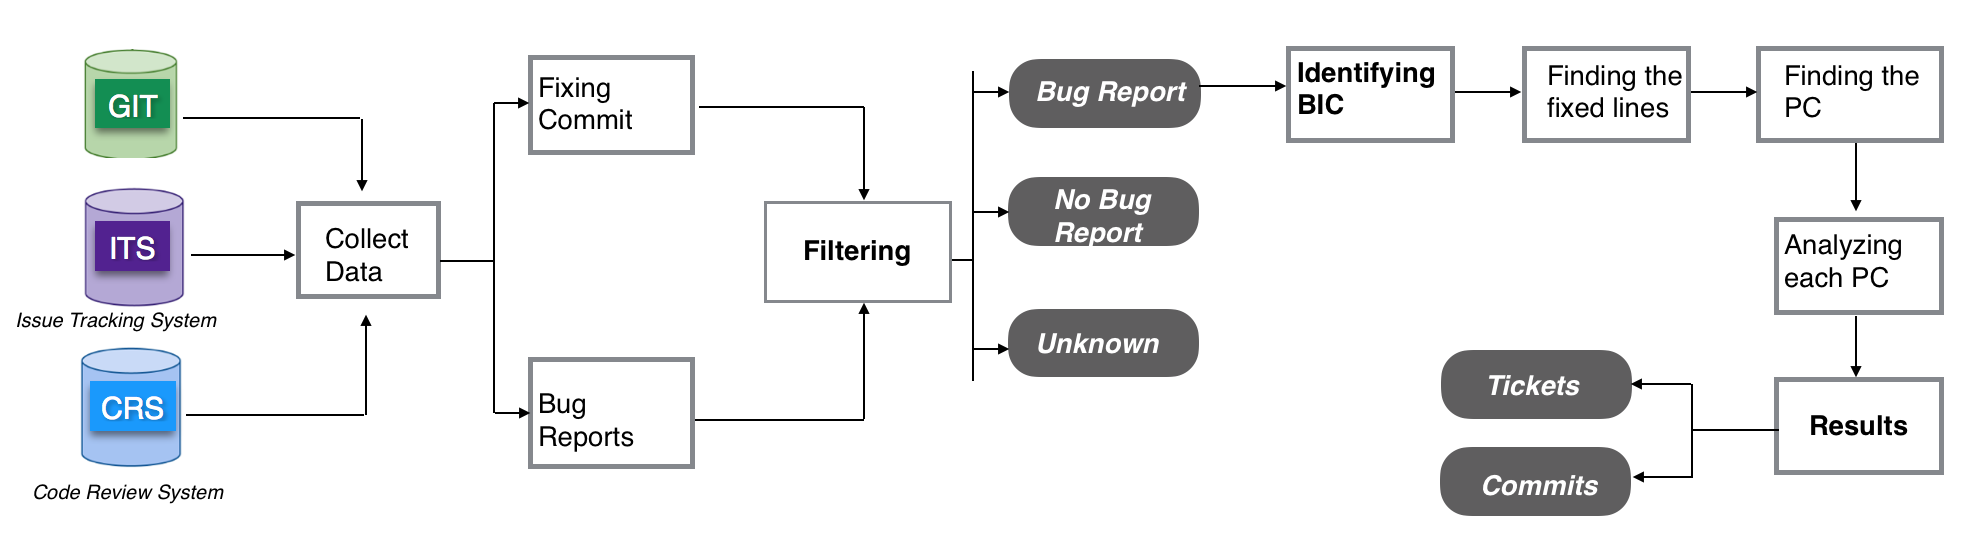
\includegraphics[width=\columnwidth]{diagram.png}
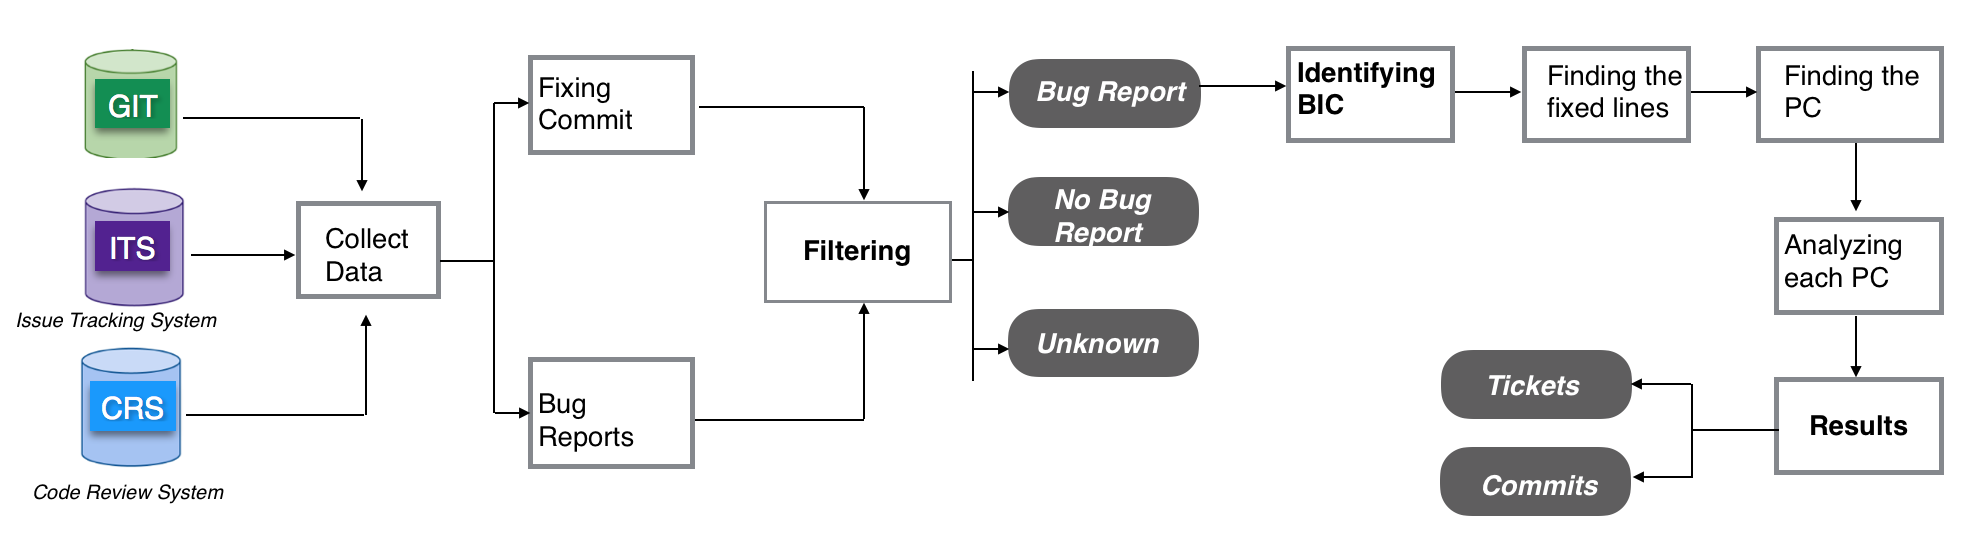
\includegraphics[height=2.5cm]{diagram.png}
\caption{Overview of the steps involved in our analysis. \emph{PC} refers to the immediately previous commit of a fixed line }
\label{fig:diagram}       % Give a unique label
\end{figure}

\subsection{Identifying the Bug introducing change of a ticket}
\label{sec:methodologySS}

The income of this stage is a set of bug report tickets extracted randomly from the issue tracking system.
All these tickets have to be closed and have a fixed commit committed and merged in the code source of the project to be able to follow the methodology described in this section.

\subsubsection{Finding the lines which fixed the bug}

We identify the commit that fixed the bug from the information of the bug fix commit (BFC), finding the lines that this commit added, modified or deleted and filtering out those lines that are not code.
	
\subsubsection{For each of those lines, identify what commit added or modified or deleted last these lines}

Each line touched by the BFC has only one previous commit, we will refer to such commits as $pc$.
This $pc$ could be the same or could be different in such lines. Thus, the result of finding the $pc$ of the bug is the $PC$ set, which could be a set of one or more $pc$. FIXME: este párrafo no queda nada claro. En este párrafo quería decir que cada BFC tiene una o mas lineas, cada una de esas lineas tiene un único pc, pero cada pc de cada línea en el BFC puede ser el mismo o puede ser distinto, por tanto como resultado tenemos un conjunto de pc's llamado PC SET.

\subsubsection{Each of these $pc$ (and its previous commits) is analyzed to determine whether it was the bug introduced change}

This analysis uses information from the BFC log and the ticket description, as well as from the log and commit changes of the $pc$.

At the end of this step we have --for each ticket analyzed-- two outcomes:
\begin{itemize}
	\item A Bug Introducing Change (BIC) does not exist: Some tickets describe a bug, but this bug was not inserted by a $pc$ or some previous commit to these $pc$, therefore there is no BIC. We will refer this set of tickets as \textit{``No BIC''}.
	\item A BIC exists: there is a BIC, it could be the $pc$ to the changed lines by the BFC or another commit that might be in the chain of previous changes of such lines or in other part of the project. We will refer this set of tickets as \textit{``BIC''}. 
\end{itemize}

\section{Evaluation} 

We have validated our methodology analyzing tickets from two different Open Source projects: \texttt{ElasticSearch} and \texttt{Nova}.
Filtering was only necessary in the case of \texttt{Nova}, as \texttt{Launchpad} does not distinguish between bug reports and other issues.
Two researchers were involved in this process, who analyzed each ticket independently.
For \texttt{ElasticSearch}, we relied on its strong policy of bug labeling.
We then manually analyzed tickets (that contain bugs, as a result from the filtering) to identify the BIC in both projects.

Our aim is to address some limitations of the SZZ approach by identifying the exact location of the BIC and understanding the reasons why a previous commit may not induce the fix. 
Hence, we introduce a new concept: the \emph{First Failing Commit (FFC)}, which is the suspicious commit to be the bug introducing commit and ideally it is located using a test case.
This concept helps to fill the scenario where lines were correct at the time of introduction but at some point a change caused that these lines become buggy, causing the bug.
The FFC might be identified by using the check test idea, where a test is passed to all previous commits until it find the first that fails.
We will refer to this commit as the FFC.


Figure~\ref{fig:test} shows the check test idea.
We are able to find the FFC based on the idea of having an omnipotent view. 
Thus, the test is passed to all previous commits looking for the one that fails.
If found, we will be consider it as a candidate for the BIC.

\begin{figure}[ht]
\centering
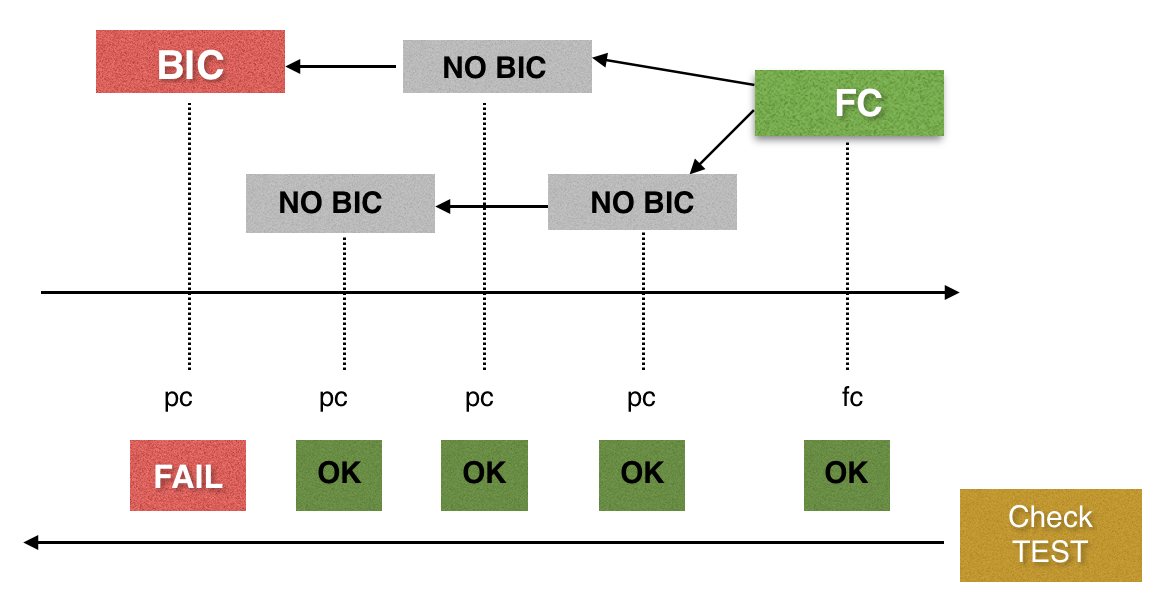
\includegraphics[height=4cm]{testrecursive.png}
\caption{Example of how we could find a candidate commit to be the  bug inducing change. Each version passes or not a test written after fixing the bug in the FC (fixing commit).}
\label{fig:test}      
\end{figure}


%\subsection{For each of these $pc$ is analyzed to determine whether it was the bug introduced change and the SZZ algorithm could found it }
%
%At the end of this step we have two outcomes for each commit analyzed based on the main assumption done by SZZ algorithm \cite{sliwerski2005changes}:
%\begin{itemize}
%	\item Founded by SZZ: The algorithm is able to locate the $pc$. It could be a true positive, $ pc == BIC $, or a false positive,$ pc \not= BIC $.
%	\item No Founded by SZZ: The algorithm is not be able to locate the $pc$ but the BIC exists, this could be when the BFC only added new lines due to some of the $pc$ forgot added. Or maybe, the algorithm is not be able to locate the $pc$ because it belongs to other part of the code or because there is any BIC.
%\end{itemize}


\subsection{For each of the tickets, could the hypothetical recursive test find the BIC as the FFC?}

At the end of this step we have two main groups for each FFC identified:
\begin{itemize}
	\item Group 1: The bug has been always there. Then, the FFC is the first commit in the project, and the test will always fail.
	\item Group 2: The FFC can be found using the test. Thus, we may have two possibilities: (a) The test fails as we expected because the failure was due to a change in other part of the code that affects the code fixed or the fixed line(s) cannot be checked before because they didn't exists. (b) The FFC is the BIC, the test fails because a previous change (the previous commit or an older commit) injected the bug.
\end{itemize}

\section{Results}
\label{sec:results}

We have analyzed 60 random tickets from the two projects, determining if the lines changed to fix a bug were the cause of the bug, and identifying whether a previous commit(s) is the BIC or not.
Thus, after finding the lines which fix the bug in the 60 tickets in \texttt{Nova} and \texttt{ElasticSearch}, we classified the tickets into two different sets, the \textit{``BIC''} set and the \textit{``No BIC''} set.
In addition, each previous commit also was classified into one of following sets: \textit{``FFC''} and \textit{``NO FFC''}.

From the 60 tickets analyzed in \texttt{Nova}, 72\% were classified into BIC group and 28\% into NO BIC group.
The number of commits analyzed at the line level was 141 and only in 30\% of the cases those commits were the FFC. 
Finally in 22\% of the cases the FFC was the BIC.

On the contrary, from the 60 bugs in \texttt{ElasticSearch}, the number of tickets classified into set BIC was higher: 75\%.
However, the set of NO BIC was a little bit lower, 25\%.
The number of commits analyzed at line level was 132 and only in 35\% of the cases those commits were the FFC.
Finally in 29\% of the cases, the FFC was the BIC.


Additionally, in those cases where the ticket does not present a BIC, we are able to present a short classification of the main reasons:
\begin{itemize}
  \item Changes to APIs, such as the addition of an argument. 
  \item Updates done, such as changes in the operating system, packages or requirements.
\end{itemize}

In any case, our research shows evidence that assuming that the $pc$ is where the cause of a bug can be found does not hold for a significant fraction of bugs.
The most common reasons for the $pc$ was neither a FFC or a BIC in the projects are:

\begin{itemize}
  \item Variable renaming.
  \item Changes done by the BFC in a clean line.
  \item Refactoring of the code in some lines.
  \item Grammar errors, dragged from former commits.
\end{itemize} 
%
%\begin{table}[!t]
%\renewcommand{\arraystretch}{1.3}
%\caption{Number of previous commit per ticket in each of the two projects analyzed, line level}
%\label{tableI}
%\centering
%\begin{tabular}{|c||c||c|c|c|}
%\hline
% & Nova(L) & ES(L)& Nova(T) & ES(T) \\
%\hline
%BIC & 40(73\%) & 38(68\%)& 40(73\%) & 38(68\%)\\
%\hline
%NO BIC & 15 (27\%) & 18 (32\%)& 15 (27\%) & 18 (32\%)\\
%\hline
%Founded & 109 (90\%) & 116 (90\%)& 128(85\%) & 132(87\%)\\
%\hline
%No founded  & 12 (10\%) & 13 (10\%)& 23(15\%) & 19(13\%)\\
%\hline
%True + & 49 (45\%) & 48 (41\%)& 61(48\%) & 48(36\%)\\
%\hline
%False + & 54 (50\%) & 64 (55\%)& 67(52\%) & 73(55\%)\\
%\hline
%\end{tabular}
%\end{table}

\section{Conclusion}

The empirical study we have performed with some bug reports from \texttt{Nova} and \texttt{ElasticSearch} has shown that for a large fraction of the analyzed tickets, around 25\%, no BIC has been identified.
So, in those tickets that present a BIC, the implicit assumption that bugs were introduced in the previous commit does not hold at least in 70\% of them.

Our study also shows that even when we are sure that some previous change introduced the bug in the line, only in some cases the $pc$ is the bug introducing change. %In other cases, the $ipc$ is not the bug introduce change and the best method to prevent these cases is the token level. And finally in the rest of cases, we are unable to locate the bug introduce change because of the several changes suffer by the code.

In many cases, we have identified which ones are the changes that actually introduced the bug, which could be useful to improve the accuracy of tools and models developed to prevent bugs.
Also, software developers can benefit from identifying where the bug was inserted, improving their processes.

Once we have found that at least in two projects, implemented in different programming languages, the $pc$ is in many cases not the bug introduction change, it makes sense to explore, as future work, to which extent this occurs in other projects, studying a higher number of tickets.


\begin{thebibliography}{1}

\bibitem{sliwerski2005changes},{\'S}liwerski, Jacek and Zimmermann, Thomas and Zeller, Andreas,When do changes induce fixes?,Proceedings of the 2005 International Workshop on Mining software repositories,1--5,2005,ACM
\bibitem{williams2008szz},Williams, Chadd and Spacco, Jaime, "Szz revisited: verifying when changes induce fixes", Proceedings of the 2008 workshop on Defects in large software systems, 32--36,2008,ACM
\bibitem{izquierdo2011developers},Izquierdo-Cortazar, Daniel and Capiluppi, Andrea and Gonzalez-Barahona, Jesus M, Are Developers Fixing Their Own Bugs?: Tracing Bug-Fixing and Bug-Seeding Committers,
  International Journal of Open Source Software and Processes (IJOSSP),23--42,2011
\bibitem {pan2009toward},Pan, Kai and Kim, Sunghun and Whitehead Jr, E James,Toward an understanding of bug fix patterns,Empirical Software Engineering,286--315,2009,Springer
\bibitem {altman1968financial},Altman, Edward I,Financial ratios, discriminant analysis and the prediction of corporate bankruptcy,The journal of finance,589--609,1968,Wiley Online Library
\bibitem{fejzer2015supporting},Fejzer, Miko{\l}aj and Wojtyna, Micha{\l} and Burza{\'n}ska, Marta and Wi{\'s}niewski, Piotr and Stencel, Krzysztof,Supporting Code Review by Automatic Detection of Potentially Buggy Changes,473--482,2015,Springer
\end{thebibliography}




% that's all folks
\end{document}


